\ifx\allfiles\undefined

	% 如果有这一部分另外的package,在这里加上
	% 没有的话不需要
	
	\begin{document}
\else
\fi
    \chapter{非线性规划}
    \section{非线性规划问题与数学模型}
    \subsection{非线性规划问题的定义}
    
\begin{dfnbox}{非线性规划}{amznotes}
    如果目标函数或约束条件方程中存在任何非线性因子,则问题\textbf{非线性规划}。
\end{dfnbox}
非线性规划具有以下几个特点:
\begin{itemize}
    \item 目标函数或约束条件方程中存在任何\textcolor{red}{非线性因子},或全部为\textcolor{red}{非线性函数}:
    \item \textcolor{red}{没有统一的、通用的解法}(这不同于线性规划,它有单纯形法作为通用解法),目前各种解法都有自己的适用范围;
    \item 非常难以采用解析解法,更多采用\textcolor{red}{数值解法};
    \item 非线性规划的最优解不像线性规划那样在边界点达到,而是\textcolor{red}{有可能在可行域中任一点}达到;
    \item 非线性规划存在\textcolor{red}{局部极值点}和\textcolor{red}{全局极值点}之分,这一点也与线性规划不同。
\end{itemize}
\begin{dfnbox}{局部极值点}{amznotes}
    设 $x^* \in K$,如果存在某个 $\epsilon > 0$,使得有与 $x$ 距离小于 $\epsilon$ 的 $x \in K$(即 $x \in K \cap \|x - x^*\| < \epsilon$),均满足不等式 $f(x) \geq f(x^*)$,则称 $x^*$ 为 $f(x)$ 在 $K$ 上的局部极小点,$f(x^*)$ 为局部极小值。\\
    若 $x \neq x^*$ 且 $f(x) > f(x^*)$,则 $x^*$ 为严格局部极小点,$f(x^*)$ 为严格局部极小值。
\end{dfnbox}
\begin{dfnbox}{全局极值点}{amznotes}
    设 $x^* \in K$,如果对于任意 $x \in K$,都有 $f(x) \geq f(x^*)$,则称 $x^*$ 为 $f(x)$ 在 $K$ 上的全局极小点,$f(x^*)$ 为全局极小值。\\
    若 $x \neq x^*$ 且 $f(x) > f(x^*)$,则 $x^*$ 为严格全局极小点,$f(x^*)$ 为严格全局极小值。
\end{dfnbox}
两点说明:
\begin{itemize}
    \item 局部极值点和全局极值点在定义上的主要区别是点的比较范围是x*附近的一个小邻域,还是整个K域。
    \item 局部极小点可能同时是全局极小点,全局极小点同时一定是局部极小点。
\end{itemize}
\begin{figure}[H]
    \centering
    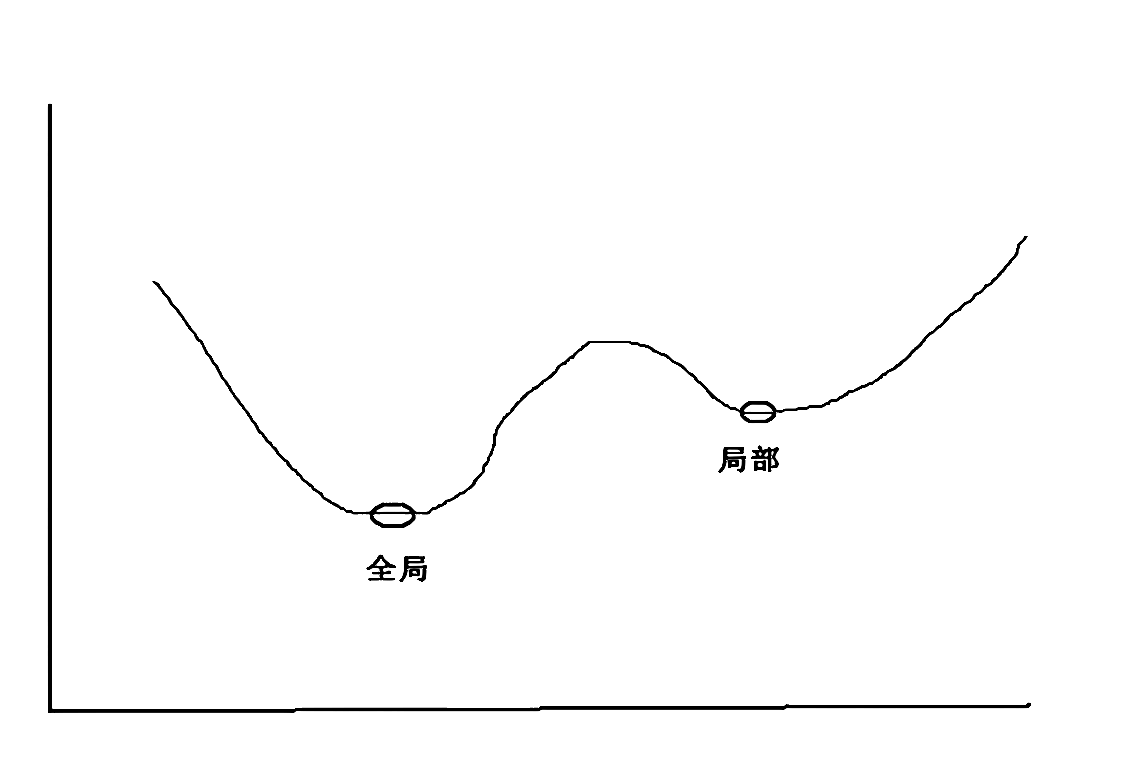
\includegraphics[width=0.5\textwidth]{./image/19.png}
    \caption{非线性规划也有局部极值和全局极值的区分}
    \label{fig:Chapter4_Temporary_Pavilion_1}
\end{figure}
\begin{figure}[H]
    \centering
    \begin{subfigure}{0.42\textwidth}
        \centering
        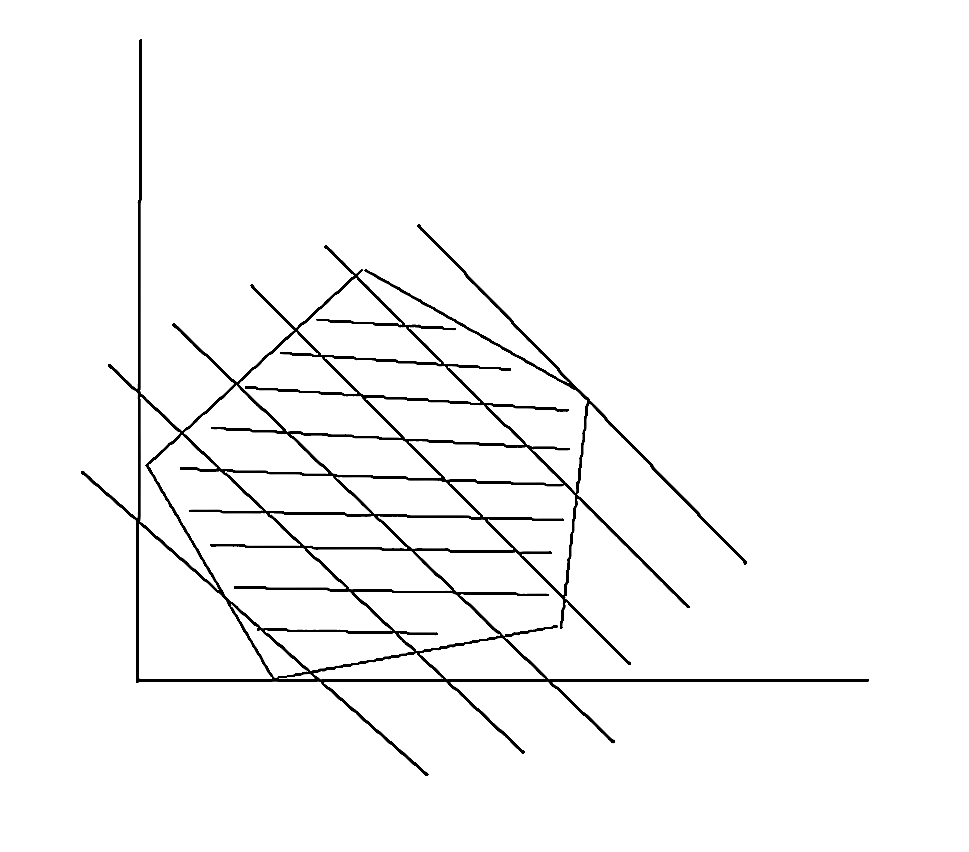
\includegraphics[width=\linewidth]{image/17.png}
        \caption{线性规划中,当目标函数取定值时,其等值几何图形为直线或平面。}
    \end{subfigure}
    \hfill
    \begin{subfigure}{0.4\textwidth}
        \centering
        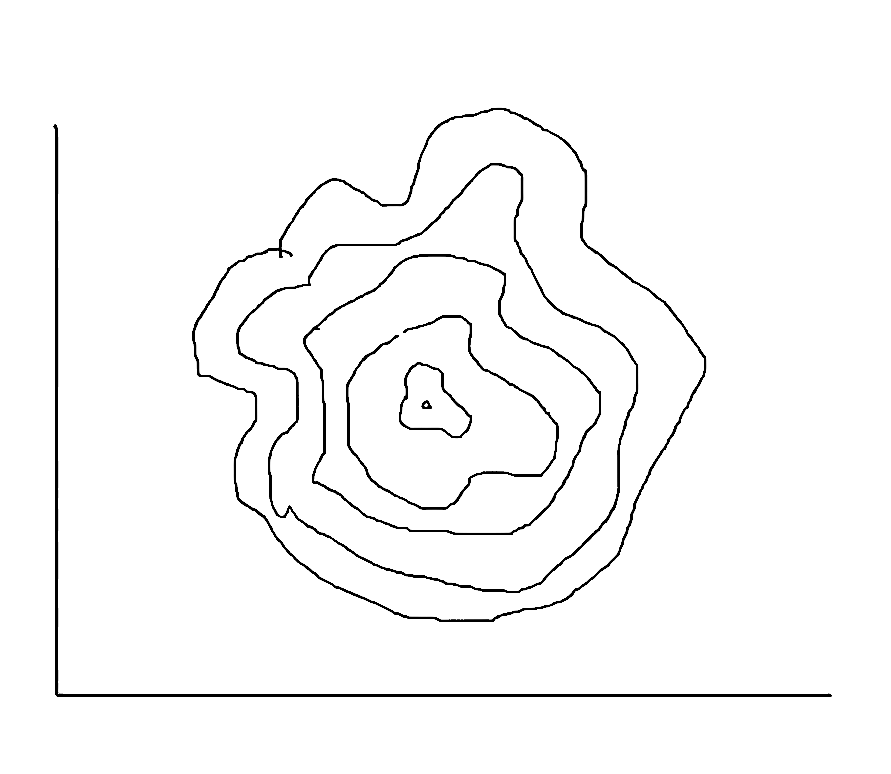
\includegraphics[width=\linewidth]{image/18.png}
        \caption{非线性规划中,等值线为规则或不规则的曲线、曲面,类似于地图上的等高线}
    \end{subfigure}
    \caption{线性规划与非线性规划的对比}
\end{figure}

\begin{exbox}{资源分配问题}
1\textbf{例:}有 A 和 B 两种资源,数量分别为 a 和 b,用于生产 n 种产品。如果 A 种资源以数量 \(x_k\),B 种资源以数量 \(y_k\),用于生产第 k 种产品,其收益为 \(g_k(x_k, y_k)\),问如何分配这两种资源用于 n 种产品的生产使总收益最大?
\\
\textbf{解:}

由题意,以 \(x_k\) 和 \(y_k\)(\(k = 1, 2, \dots, n\))为决策变量,以生产 n 种产品的总收益为目标函数,资源的总量为约束条件,则问题的优化模型为:

\[
\max z = g_1(x_1, y_1) + g_2(x_2, y_2) + \dots + g_n(x_n, y_n)
\]

约束条件:

\[
\begin{cases}
x_1 + x_2 + \dots + x_n = a, \\
y_1 + y_2 + \dots + y_n = b, \\
x_k \geq 0, \quad y_k \geq 0 \quad (k = 1, 2, \dots, n).
\end{cases}
\]
\end{exbox}

\begin{exbox}{最小圆盘问题}
    1\textbf{例:}设平面上有 $m$ 个点,找覆盖这 $m$ 个点的最小圆盘。

    \textbf{解:} 设 $m$ 个点为 $p_i, \, i = 1, 2, \dots, m$,则平面上任一点 $x$ 到这 $m$ 个点的距离最大者满足
    
    \[
    f(x) = \max_{1 \leq i \leq m} \| x - p_i \|
    \]
    
    则以 $x$ 为圆心,$f(x)$ 为半径的圆盘必覆盖这 $m$ 个点,于是问题转化为求解最小半径的圆盘问题:
    
    \[
    \min_x \max_{1 \leq i \leq m} \| x - p_i \|
    \]
    
    这是一个无约束的非线性规划问题。
\end{exbox}
\textcolor{red}{若没有约束条件,称为无约束极值问题。否则称为约束极值问题。}
\subsection{非线性规划问题的数学模型}
\begin{thmbox}{一般形式}{cool}
    \begin{align*}
        \text{max} \quad & z = g_1(x_1, y_1) + g_2(x_2, y_2) + \cdots + g_n(x_n, y_n) \\
        \text{subject to} \quad & \sum_{k=1}^{n} x_k = a, \\
        & \sum_{k=1}^{n} y_k = b, \\
        & x_k \geq 0, \ y_k \geq 0 \quad (k = 1, 2, \dots, n).
        \end{align*}
        
        \begin{align*}
        \text{min} \quad & \max_{1 \leq l \leq m} \left\{ \| x - p_l \| \right\}
    \end{align*}
\end{thmbox}
\begin{thmbox}{标准模型I}{cool}
    \begin{align*}
        \min \quad & f(x) \\
        \text{subject to} \quad & h_i(x) = 0, \quad i = 1, 2, \dots, m \quad \text{(m 个等式约束)} \\
        & g_j(x) \geq 0, \quad j = 1, 2, \dots, l \quad \text{(l 个不等式约束)} \\
        & x \in \mathbb{R}^n
        \end{align*}
        
        \bigskip
        \text{若有另一种形式,可以转化为上述形式,例如:}
        \begin{align*}
        \max \quad  f(x) \quad &\Rightarrow \quad \min (-f(x)) \\
        g_j(x) \leq 0  \quad &\Rightarrow \quad -g_j(x) \geq 0
        \end{align*}
\end{thmbox}
\begin{thmbox}{标准模型II}{cool}
    \begin{align*}
        \min \quad & f(x) \\
        \text{subject to} \quad & g_i(x) \geq 0, \quad i = 1, 2, \dots, n \quad \text{(n 个不等式约束)} \\
        & x \in \mathbb{R}^n
    \end{align*}
\end{thmbox}


\begin{notebox}{\textbf{模型 I 与模型 II 的转换:}}
\\
主要是把等式约束化为不等式约束:
\begin{align*}
    h_i(x) = 0 \quad \Rightarrow \quad \begin{cases}
        h_i(x) \geq 0 \\
        h_i(x) \leq 0 \quad \Rightarrow \quad -h_i(x) \geq 0
    \end{cases}
    \Rightarrow
    g_i(x)\geq 0 
\end{align*}
\end{notebox}
\begin{notebox}{\textbf{求解方法}}
    \\求解非线性规划问题常有两种方法:
    \begin{enumerate}
        \item \textbf{解析法}:必要条件+充分条件;
        \item \textbf{数值法}:迭代。
    \end{enumerate}
\end{notebox}


\subsection{求解非线性规划问题的解析法}
为了使用解析方法解决非线性规划问题,我们首先引出几个定义\footnote{读者在微积分或数学分析课程中中学过以上概念。如果感到有些遗忘,可以理解为“梯度”就相当于一元函数的一阶导数,“Hesse 矩阵”就相当于一元函数的二阶导数。我们在判断一元函数的极值点的时候,就是通过求一阶导为0,二阶导大于或小于0来判断是极小值或极大值的。对于多元函数也是类似的道理。}:
\begin{dfnbox}{函数的梯度}{amznotes}
    设 $x \in K \subset \mathbb{R}^n$,$f(x)$ 在 $K$ 上有一阶连续偏导数,则
    \[
    \nabla f(x) \equiv \left[ \frac{\partial f(x)}{\partial x_1}, \frac{\partial f(x)}{\partial x_2}, \ldots, \frac{\partial f(x)}{\partial x_n} \right]^T
    \]
    称函数 $f(x)$ 在 $x$ 处的\textbf{梯度}。
\end{dfnbox}
\textbf{梯度的几何意义}:
    $\nabla f(x)$ 是 $f(x)$ 在 $x$ 处增加最快或减少最快的速度,也是 $f(x)$ 的图形在 $x$ 处的陡峭程度。
\begin{dfnbox}{平稳点}{amznotes}
    若$\nabla f(x)=0$,则称$x$是$f(x)$的\textbf{平稳点}。
\end{dfnbox}

\begin{dfnbox}{海森Hesse矩阵}{amznotes}
    设 $f(x)$ 在 $K$ 上有二阶连续偏导数,则
    \[
    H(x) \equiv \begin{bmatrix}
        \frac{\partial^2 f(x)}{\partial x_1^2} & \frac{\partial^2 f(x)}{\partial x_1 \partial x_2} & \cdots & \frac{\partial^2 f(x)}{\partial x_1 \partial x_n} \\
        \frac{\partial^2 f(x)}{\partial x_2 \partial x_1} & \frac{\partial^2 f(x)}{\partial x_2^2} & \cdots & \frac{\partial^2 f(x)}{\partial x_2 \partial x_n} \\
        \vdots & \vdots & \ddots & \vdots \\
        \frac{\partial^2 f(x)}{\partial x_n \partial x_1} & \frac{\partial^2 f(x)}{\partial x_n \partial x_2} & \cdots & \frac{\partial^2 f(x)}{\partial x_n^2}
    \end{bmatrix}
    \]
    称函数 $f(x)$ 在 $x$ 处的 \textbf{Hesse 矩阵}。
\end{dfnbox}
\begin{dfnbox}{矩阵的正定性,负定性,不定性}{amznotes}
    对于对称矩阵 $A$,若对任意非零向量 $X \neq 0$,二次型为正,即 $X^T A X > 0$,则称该二次型为正定二次型,$A$ 为正定矩阵\footnote{在线性代数中,我们学习过判断正定矩阵的方法有特征值判定法(所有特征值大于0)、主子式判定法(如果所有阶的顺序主子式,即从左上角开始的子矩阵的行列式都大于0);此外,如果两个矩阵都是正定的,那他们的和也是正定的;一个正定矩阵的逆矩阵也是正定的。}。\\
    若 $X^T A X \geq 0 \Rightarrow$ 半正定\\
    若 $X^T A X < 0 \Rightarrow$ 负定\\
    若 $X^T A X \leq 0 \Rightarrow$ 半负定\\
    若既非正定,又非负定,则为不定。
\end{dfnbox}
\begin{thmbox}{定理一:极值点必要条件}{cool}
    若$f(x)$在其存在一阶连续偏导数的区域内达到局部极值点,则该极值点必为平稳点。
\end{thmbox}
此处要注意:
\begin{itemize}
    \item 该定理是必要条件,反之不一定成立,即\textcolor{red}{平稳点不一定是极值点},例如鞍点。
    \item $f(x)$在其不满足一阶连续偏导数的区域内的极值点,不一定满足定理一。
\end{itemize}
\begin{figure}[H]
    \centering
    \begin{subfigure}{0.42\textwidth}
        \centering
        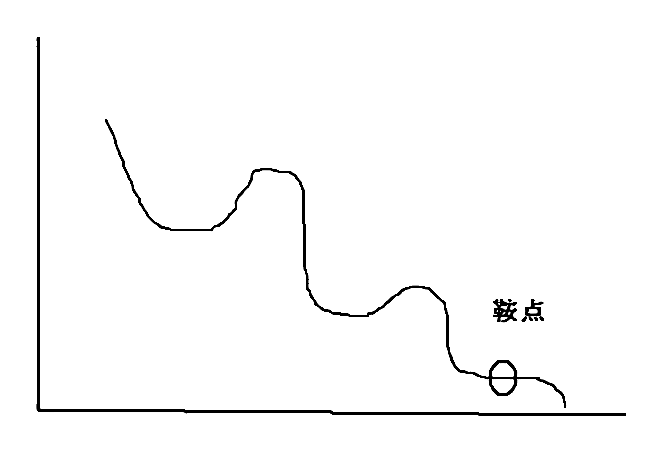
\includegraphics[width=\linewidth]{image/20.png}
        \caption{鞍点是平稳点但不是极值点}
    \end{subfigure}
    \hfill
    \begin{subfigure}{0.4\textwidth}
        \centering
        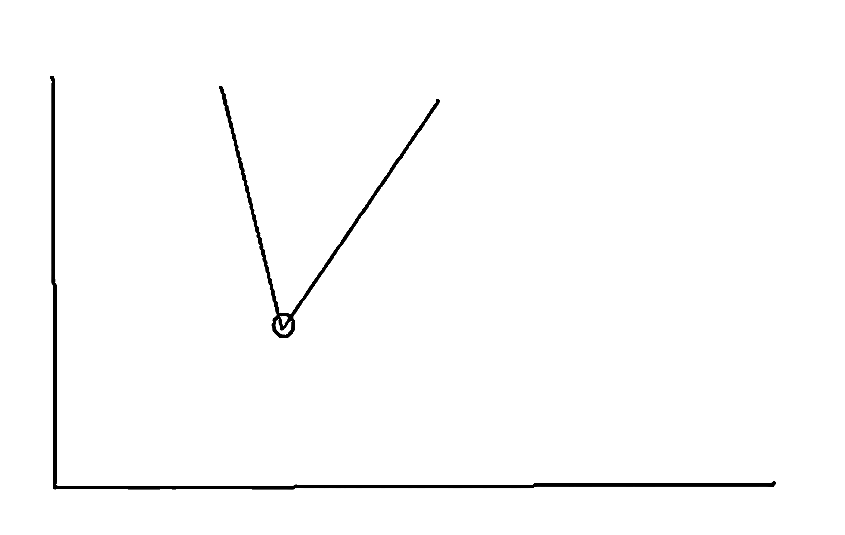
\includegraphics[width=\linewidth]{image/21.png}
        \caption{一阶偏导数不连续的极值点不一定是平稳点}
    \end{subfigure}
    \caption{定理一是必要条件的理解}
\end{figure}
为了能够正确判断极值点,我们使用定理二:
\begin{thmbox}{定理二:局部极值点判断的充要条件}{cool}
    若 $f(x)$ 在 $K$ 上具有二阶连续偏导数,并且满足:
    \begin{enumerate}
        \item $x^* \in K$ 是平稳点,即 $\nabla f(x^*) = 0$
        \item $H(x^*)$ 是正定矩阵(Hesse 矩阵)
    \end{enumerate}
    则 $x^* \in K$ 是 $f(x)$ 的严格局部极小点。
\end{thmbox}
\subsection{求解非线性规划问题的数值法}

\begin{dfnbox}{下降迭代算法}{amznotes}
    若由某算法产生的解序列 $\{ X^{(k)} \}$ 使目标函数值 $f(X^{(k)})$ 逐步减小,则称这组算法为\textbf{下降迭代算法}。
\end{dfnbox}

\begin{notebox}{\textbf{下降迭代算法}}{}
    \begin{itemize}
        \item \textbf{迭代法的基本思路:}
        \\
        初始估计 $X^{(0)}$ \quad $\xrightarrow{\text{按某种算法}}$ \quad 比 $X^{(0)}$ 更好的 $X^{(1)}$ \quad $\xrightarrow{\text{按算法}}$ \quad $X^{(2)} \cdots X^{(n)}$
        $\xrightarrow{\text{得到解序列}} \quad \{ X^{(0)}, X^{(1)}, \cdots, X^{(n)} \cdots \}$
    
        \bigskip
        若解序列收敛于 $X^*$,即,
        \[
        \lim_{k \to \infty} \| X^{(k)} - X^* \| = 0
        \]
        则称 $\{ X^{(0)}, X^{(1)}, \cdots, X^{(n)} \cdots \}$ 收敛于 $X^*$。
        \\
    \end{itemize}
\end{notebox}
几个关键问题是:
\begin{enumerate}
    \item 迭代算法的初始点 $X^{(0)}$ 的选择?
    \item 算法的设计,以当前点依据何种原则构建下一个点?
    \item 迭代算法的终止条件?
\end{enumerate}
\subsubsection{迭代法的基本步骤}
\begin{itemize}
\item \textbf{一、初值的确定}\\初值的确定没有特别的办法,很多情况下依靠经验,或求解者对问题的了解程度来确定的。初值应尽可能与可能的最优解靠得近一些。
\item \textbf{二、算法的设计}
\begin{enumerate}
    \item 选定某一初始点 $X^{(0)}$,并令 $k=0$。

    \item 确定能使 $f(X)$ 下降的搜索方向 $P^{(k)}$。

    \item 从 $X^{(k)}$ 出发行,沿方向 $P^{(k)}$ 确定迭代步长 $\lambda_k$。

    \item 确定,产生下一个迭代点 $X^{(k+1)}$,
    \[
    X^{(k+1)} = X^{(k)} + \lambda_k P^{(k)}.
    \]
    \item 检查新点$X^{k+1}$是否为极小点,或近似极小点,或满足规定的停止条件。
    \begin{itemize}
        \item 若是,则停止迭代;
        \item 否则,令 $k=k+1$,转(2)继续进行迭代。
    \end{itemize}
\end{enumerate}
\textcolor{red}{关键在于如何选取搜索方向 $P^{(k)}$ 和步长 $\lambda_k$}\footnote{各种迭代方法的差异主要就体现在这两者的选定上。}。
\\方向的确定相对困难,但很重要,避免南辕北辙。
\\步长的确定可见\hyperref[确定迭代步长的一维搜索方法]{确定迭代步长的一维搜索方法}和\hyperref[确定迭代步长的黄金分割法]{确定迭代步长的黄金分割法}。
\item \textbf{三、算法的结束条件}
\begin{itemize}
    \item 若算法优秀且收敛的极限值确为最优解,则能通过选代找到最优解。
    \item 若迭代步数有限,只能找到近似解,当满足所要求精度时,即停止迭代。
\end{itemize}
常用以下几个方法:
\begin{enumerate}
    \item \textbf{两次迭代值的绝对误差}
    \[
    \| X^{(k+1)} - X^{(k)} \| < \varepsilon_1
    \]
    \[
    | f(X^{(k+1)}) - f(X^{(k)}) | < \varepsilon_2
    \]

    \item \textbf{两次迭代值的相对误差}
    \[
    \frac{\| X^{(k+1)} - X^{(k)} \|}{\| X^{(k)} \|} < \varepsilon_1
    \]
    \[
    \frac{| f(X^{(k+1)}) - f(X^{(k)}) |}{| f(X^{(k)}) |} < \varepsilon_2
    \]

    \item \textbf{梯度条件}
    \[
    \| \nabla f(X^{(k)}) \| < \varepsilon
    \]
\end{enumerate}
\end{itemize}

\subsubsection{确定迭代步长的一维搜索方法}
\label{确定迭代步长的一维搜索方法}
\begin{notebox}{\textbf{一维、确定步长的三种方法}}
    \begin{enumerate}
        \item \textbf{恒定步长:} 步长每次不变,计算简单,但效果较差。

        \item \textbf{变步长:} 每次人工调整步长,效果较好,但实施麻烦,且需具备较多的经验。

        \item \textbf{最速下降步长:} 使沿搜索方向使目标函数值下降最多、最快,即沿射线 $X = X^{(k)} + \lambda P^{(k)}$ 求使目标函数 $f(X)$ 的极小,
        \[
        \lambda_k : \min f(X^{(k)} + \lambda P^{(k)}),
        \]
        由于这种方法是以$\lambda$为变量的元函数 $f(X^{(k)} + \lambda P^{(k)})$ 的极小点 $\lambda_k$,故称为一维搜索,这种确定的步长为\textbf{最佳步长}。
    \end{enumerate}
\end{notebox}
以下面这个草图为例,从零点出发,方向确定为横轴正方向了,如果在横轴上走出红色的步长,纵轴下降红色的部分;但是如果在横轴走出蓝色的步长,纵轴下降的部分就会更大。这就是先确定方向,沿着搜索方向使目标函数值下降最多。
\begin{figure}[H]
    \centering
    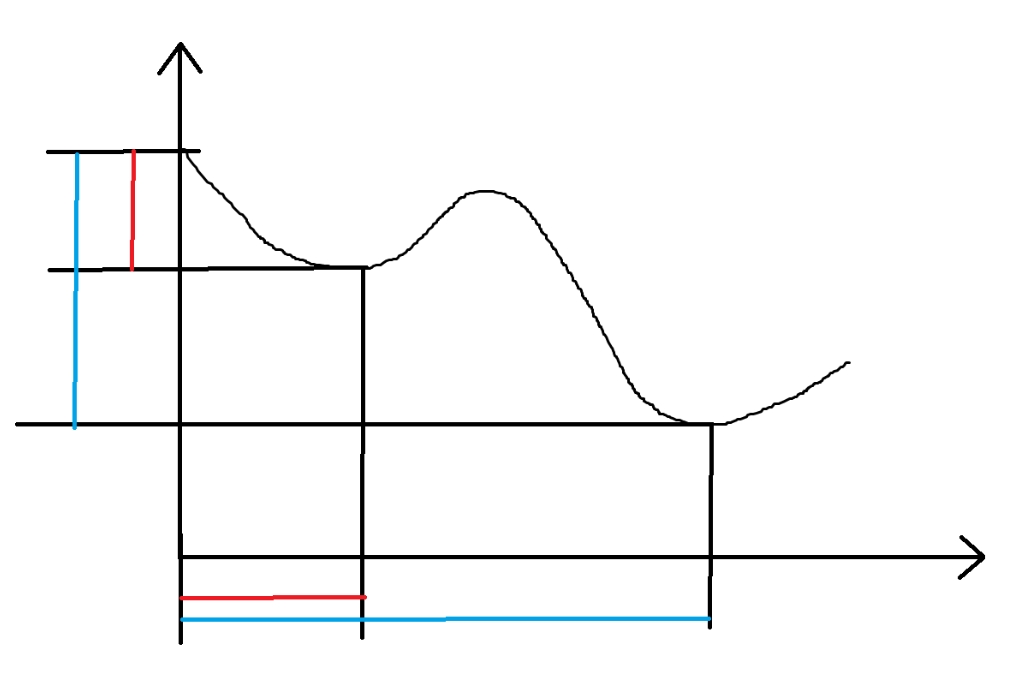
\includegraphics[width=0.35\textwidth]{./image/22.png}
    \caption{最速下降步长}
    \label{fig:Chapter4_Temporary_Pavilion_1}
\end{figure}
实际上,读者可能会想到,如果我们每次都要实时计算步长,岂不是降低了效率吗?这个问题是有道理的,请看下面的流程图:
\begin{figure}[H]
    \centering
    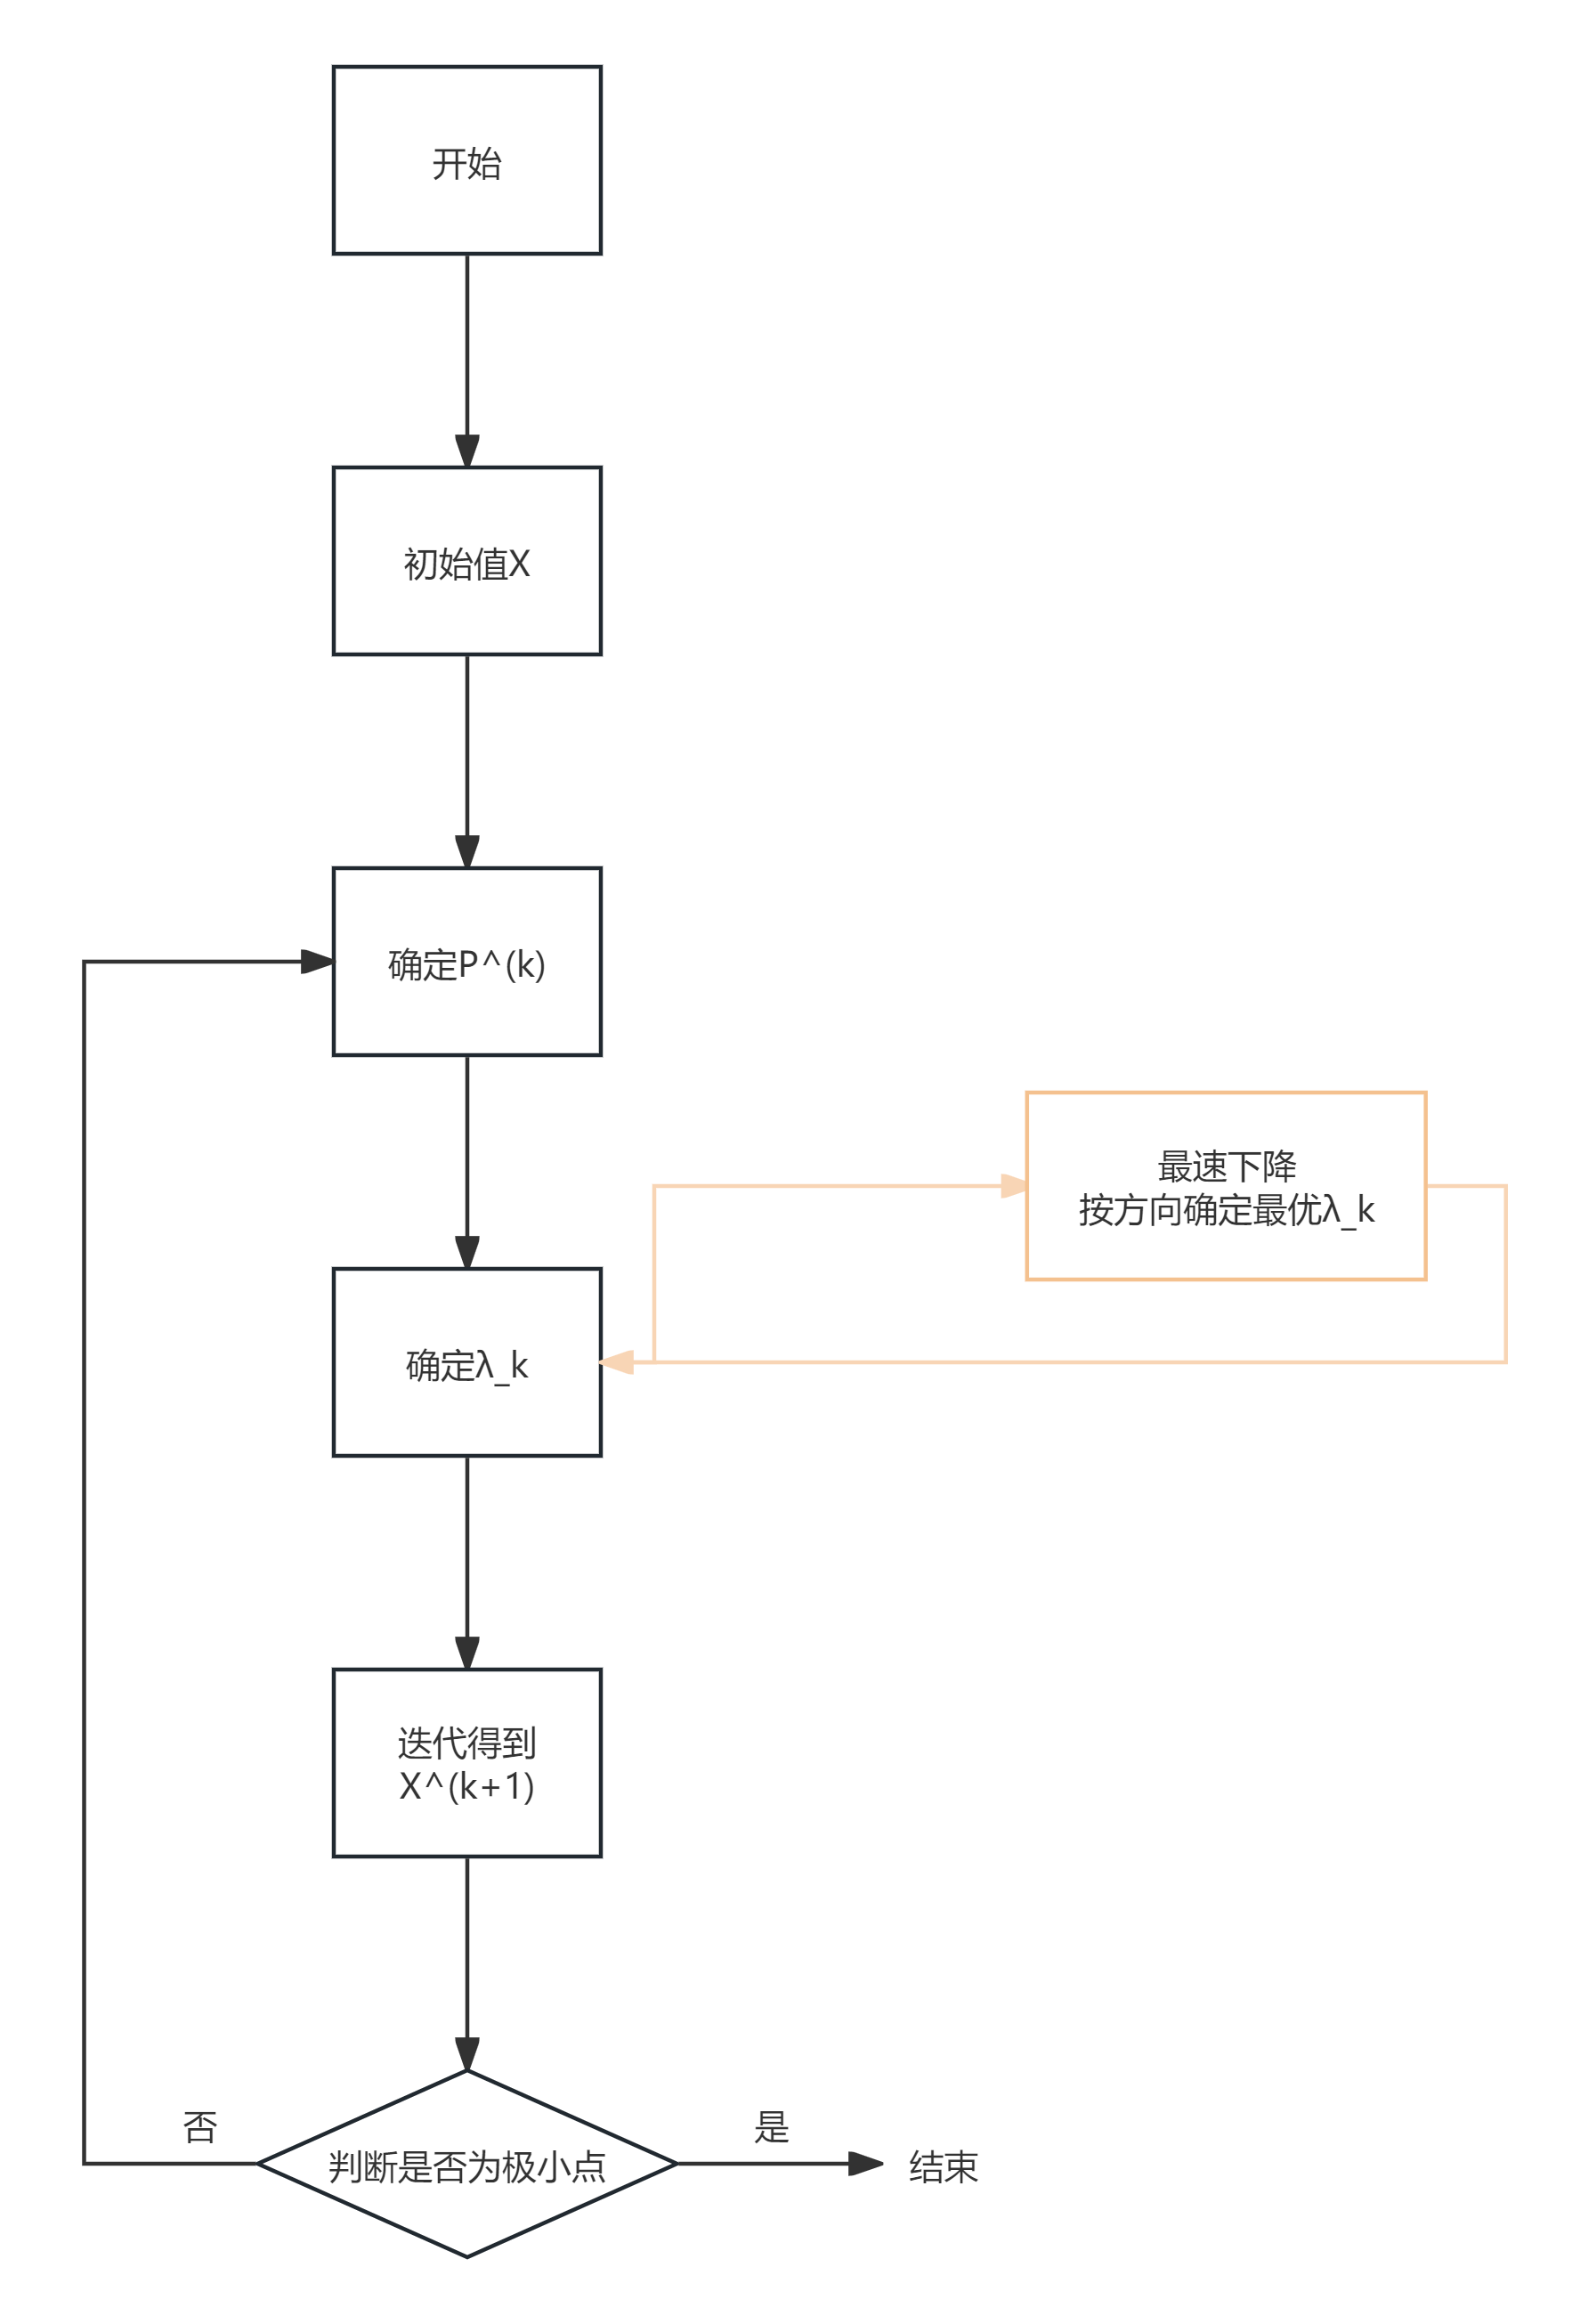
\includegraphics[width=0.6\textwidth]{./image/23.png}
    \caption{流程图}
    \label{fig:Chapter4_Temporary_Pavilion_1}
\end{figure}
引入\textcolor{orange}{橙色环节}之前,可能需要迭代100次,每次执行1秒;引入橙色环节之后,可能需要迭代50次,每次执行2秒。所以总的时间谁多谁少很难说了。因此我们想到,是否有办法在迭代过程中,既能带有最优步长的色彩,计算又不过于复杂?
\subsubsection{确定迭代步长的黄金分割法(0.618法)}
\label{确定迭代步长的黄金分割法(0.618法)}
\begin{notebox}{\textbf{黄金分割法(0.618 法)}}{}
    \\作为一种计算更简便的方法,黄金分割法在区间缩短效率上近似斐波那契法。
    \[
    x_k' = a_{k-1} + 0.382 [b_{k-1} - a_{k-1}]
    \]
    \[
    x_k'' = a_{k-1} + 0.618 [b_{k-1} - a_{k-1}]
    \]
    其中 $x_k'$ 和 $x_k''$ 分别是 $[a_{k-1}, b_{k-1}]$ 区间内的两个点,$0.382$ 和 $0.618$ 是黄金分割法的两个常数。
    可以这么理解:$x_k'$其实是$a_k$,$x_k''$其实是$b_k$,新的$\lambda_k$为$b_{k}-a_{k}$,旧的$\lambda_{k-1}$为$a_{k-1}-b_{k-1}$ 
\end{notebox}

\section{无约束非线性规划问题的解}
    \section{约束非线性规划问题(约束极值问题)}
    \section{案例分析}


\ifx\allfiles\undefined
	
	% 如果有这一部分的参考文献的话,在这里加上
	% 没有的话不需要
	% 因此各个部分的参考文献可以分开放置
	% 也可以统一放在主文件末尾。
	
	%  bibfile.bib是放置参考文献的文件,可以用zotero导出。
	% \bibliography{bibfile}
	
	end{document}
	\else
	\fi